\section{Installing NOOBS}
\label{sec:NOOBS}

	On most Raspberry Pis, we usually run an operating system called Raspbian, which is a variant of the GNU/Linux operating system.
	
%	\begin{aside}
%		Because the ARM processor in the Raspberry Pi is similar those found in billions of smartphones around the world, there are lots of other operating systems to choose from, such as other Linux distributions like Ubuntu or Arch, mobile OS's such as Android, and even a variant of Windows 10.
%	\end{aside}
	
	Raspbian can be quite tricky to install on an SD card, so a piece of software called NOOBS is provided to do most of the work for us.
	
	Many Raspberry Pi retailers sell SD cards with NOOBS pre-installed, but if you have chosen to use or purchase a blank MicroSD card, installing NOOBS yourself is straightforward.

	\subsection{Download and Install}
	
	The following instructions are for Windows 10, but should be fairly similar to most operating systems, including other versions of Windows, and MacOS.
		
	
		\begin{enumerate}[nosep]
			\item \textbf{Format your MicroSD card as a FAT file system.}
			
			On windows, right click on the SD card in the file explorer, and click `Format...'.	Most settings can be left as normal, ensure the file systems is set to `FAT32', then press Start.
			
			\begin{center}
				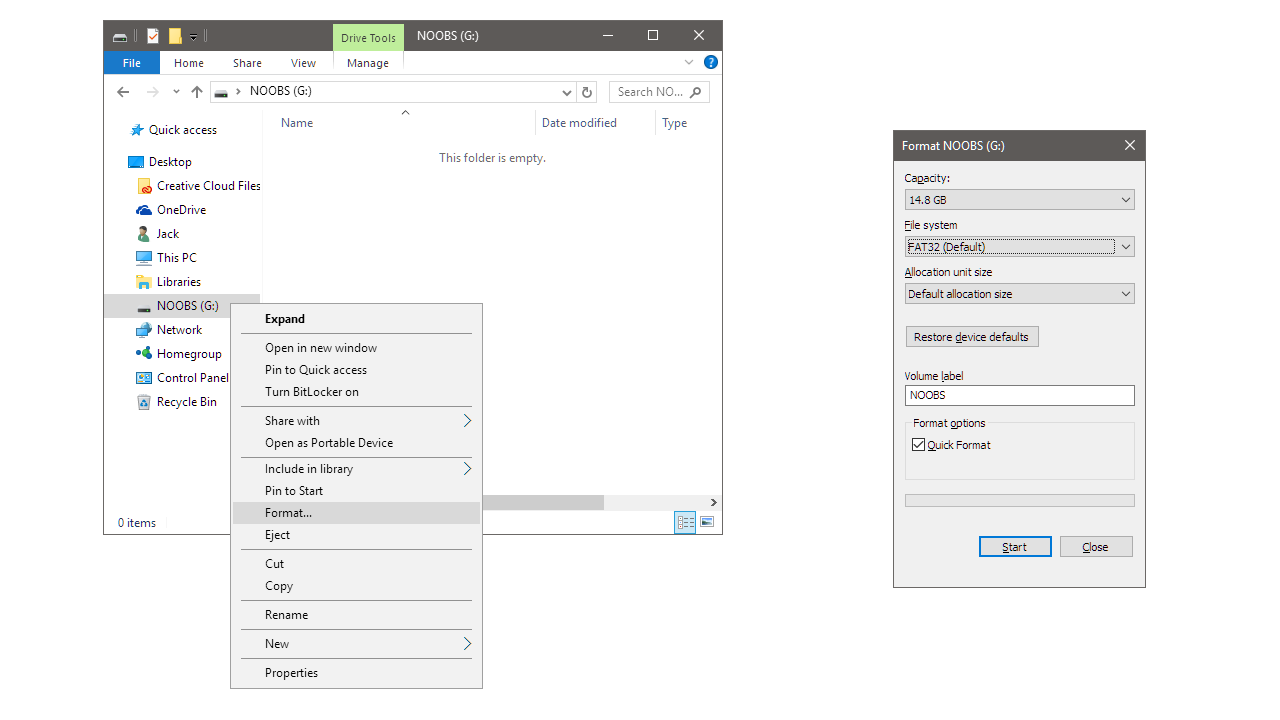
\includegraphics[width=1\linewidth]{McrRaspJam/000_IntroToPi/2_NOOBS/noobs2}
			\end{center}
			
			\item \textbf{Download the latest version of NOOBS} from \url{https://www.raspberrypi.org/downloads/}
			
			Click the `Download ZIP' button of NOOBS on the following page.
			
			\begin{center}
				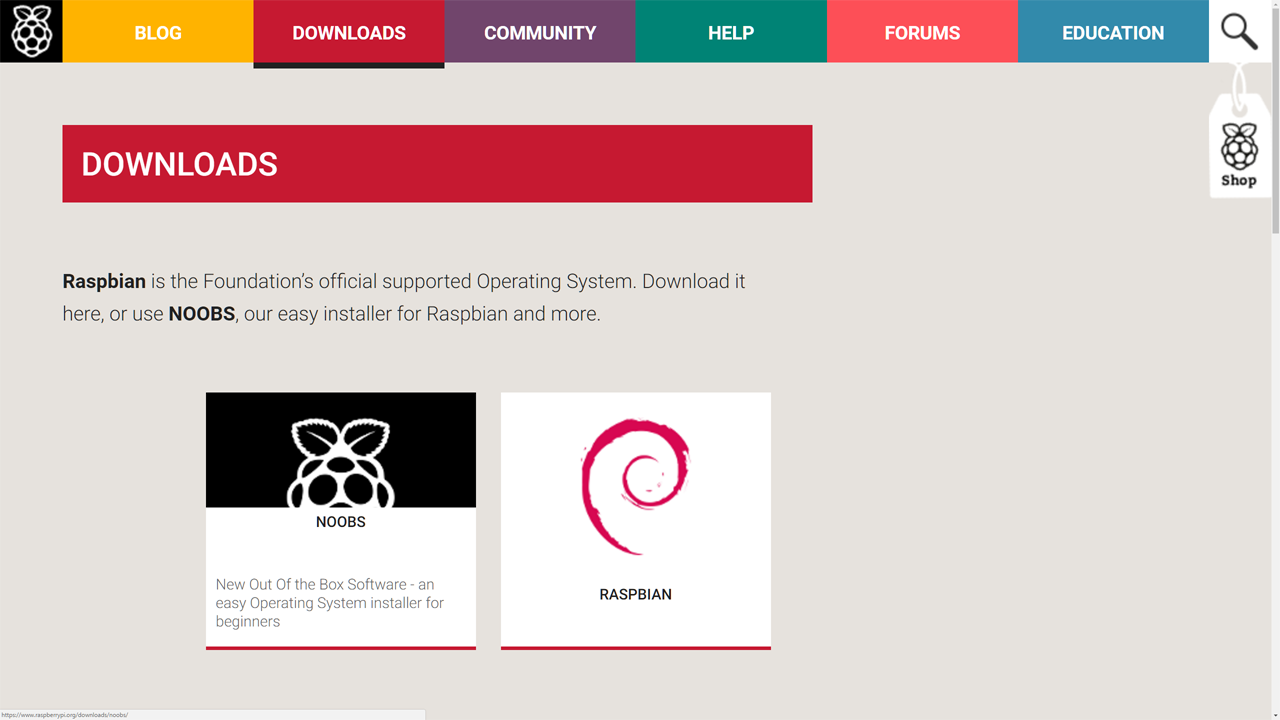
\includegraphics[width=0.8\linewidth]{McrRaspJam/000_IntroToPi/2_NOOBS/noobs1}
			\end{center}
			
			\item \textbf{Extract the downloaded NOOBS ZIP file onto the SD card}.
			
			On windows, you can right click and `Extract All...' to the drive letter of your SD card e.g. `G:\textbackslash'.
			
			\begin{center}
				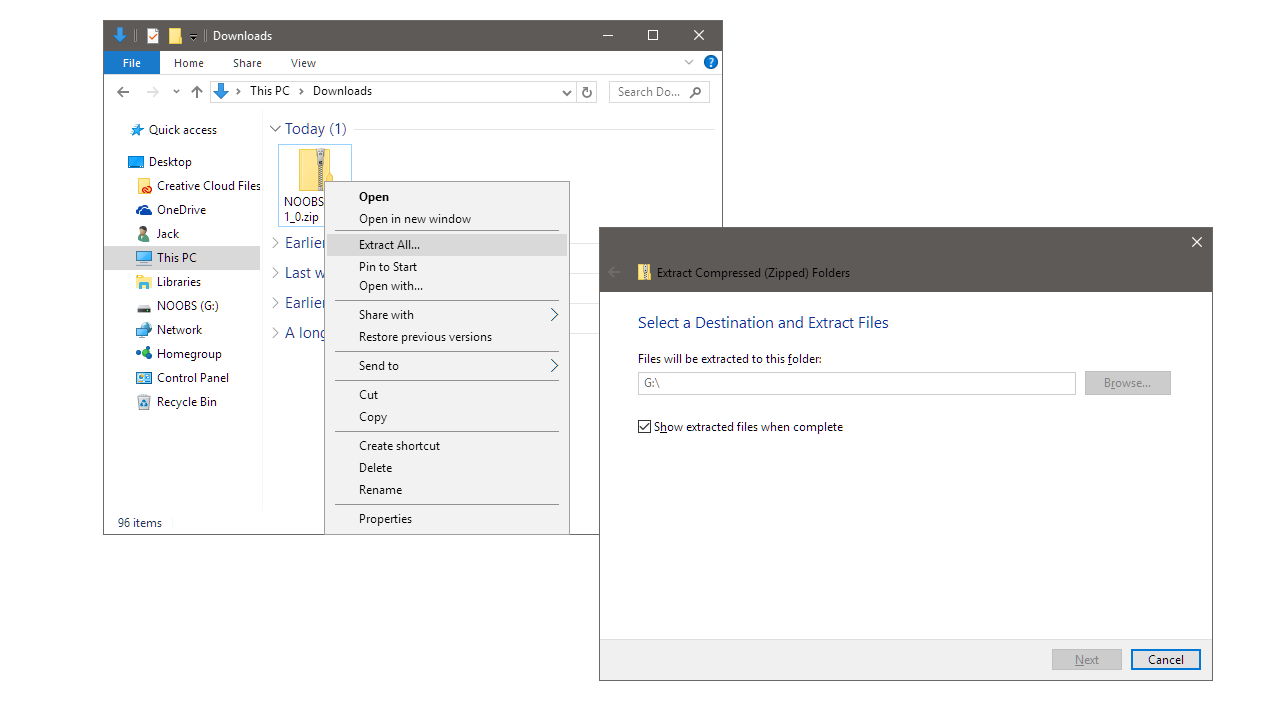
\includegraphics[width=1\linewidth]{McrRaspJam/000_IntroToPi/2_NOOBS/noobs3}
			\end{center}
		\end{enumerate}
		
		Ensure the files are extracted to the top level of the SD card, and not inside a subfolder.
		
		\subsection{Booting and Installing Raspbian}
		
		Once you have a NOOBs card set up, you can boot your Pi with it. You should see a screen like the following.
		
		\begin{center}
			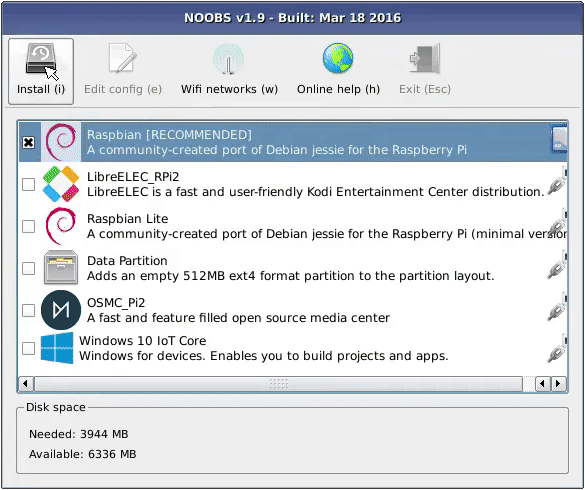
\includegraphics[width=0.8\linewidth]{McrRaspJam/000_IntroToPi/2_NOOBS/noobs5}
		\end{center}
		
		Select Raspbian (which is the only option when offline) and click install. Follow through any prompts until you reach a loading screen.
		
		The rest of the process is automatic -- and very slow -- so now is the time to find something to do for the next 20 minutes!
		
		
	
